\author{Bautrelle Fotso}
\graphicspath{ {./src/chapters/developer/media/}}

\chapter{Artificial Intelligence}
The aim of this part of the project is to build models, which will automatically recognize handwritten characters such as letters and numbers in exam 
exercises. This contributes to a faster correction of exams and enables the teacher to be more efficient by saving time.
This task can not be possible without Artificial Intelligence (AI).
In the book \emph{``State-of-the-Art Approach to Artificial Intelligence``}, the autor 
Soumyajit Goswani defines Artificial Intelligence as "(...) a computer system, which can accomplish responsibilities 
that usually need human acumen."(\cite{[1]}, p.2). 
This means, artificial intelligence can help to perform many activities like speech recognition, translation from one language to 
another, image classification and more. 
The application domain of AI matching with the objective of this project is the image classification based on machine learning.
Machine learning is a subset of AI that requires no human intervention to perform a task related to a given 
input data from which it learned.(\cite{[1]}, p.2)
One of the main categories of machine learning is deep learning, used to recognize handwritings. \hfill \break


\section{Datasets}
Datasets are the basic elements in the building process of models.
For the recognition of characters some predefined images are required. 
These images are all grouped as one to form a dataset.
Some datasets are already available on websites. 
However, it can happen that the datasets found on internet do not match the requirements of a project.
In this case, a custom dataset is needed and must be created.
\noindent
Both types of datasets mentioned above have been used for this project and each of them is explained in the next section of this chapter.

\subsection{Ready-for-use datasets}
The ready-for-use datasets are kaggle A-Z and EMNIST datasets. 
They are all available on the website \url{www.kaggle.com}(\cite{[2]}) and stored in a csv format. 
Both datasets derives from a larger dataset known as the NIST special
database 19, which contains digits, uppercase and lowercase handwritten letters. 
Each dataset has a training and a test set. 
The training set is used to train a network to recognize characters.
The test set on the other hand is used after the training of the network to validate his recognition performance against new characters. 
The EMNIST and the kaggle A-Z Datasets used in this project can be classified as follows:

\begin{itemize}
    \item Numerical datasets
    \item Alphabetical datasets
    \item Alpha-numerical datasets.
  \end{itemize}

\subsubsection{Numerical datasets}
Numerical datasets are used exclusively to recognize numbers. 
This type of dataset provides balanced handwritten digits from 0 to 9. 
"Balanced" means each class(from 0 to 9) contains the same number of images in the dataset. 
In an example of exercise, the pupil is asked to count and write down the exact number of balls in a box. 
The answer should be written in the space provided for this purpose.
This handwritten answer will be predicted by using a particular model, resulting from the training of a built network on the numerical dataset. 
To realize this feature, two main datasets of this categorie have been used:
\begin{itemize}
    \item MNIST dataset
    \item EMNIST-digits dataset.
  \end{itemize}

\noindent
The MNIST dataset has fewer data than the EMNIST-digits dataset and is an excellent dataset to get started in 
deep learning. 
The MNIST dataset contains 60.000 images in its training set and 10.000 images make up its test set. 
Each MNIST image has a size of 28x28 pixels and it can be resized according to the requirement of each project.
For this project the image was resized only for a verification purpose, because the size of 28x28 pixels was required. \hfill \break

\noindent
The fact that EMNIST-digits has more data, provides many possibilities 
to perform predictions on a wide range of differently handwritten numbers.
It also consists of a training and test set with 240.000 and 40.000 images respectively. \hfill \break

\noindent
A sample of both are shown in figure(\ref{Abb:digits_sample}) 
\begin{figure}[htb]
	\centering
	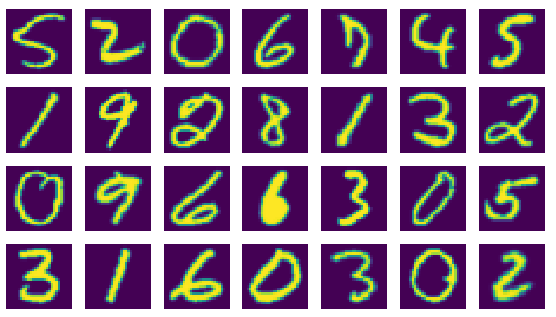
\includegraphics[scale=0.4]{digits_dataset}
	\caption[Digits datasets]{MNIST and EMNIST Digits}\label{Abb:digits_sample}
\end{figure}


\subsubsection{Alphabetical dataset}
For the purpose of this project, two datasets were used for the recognition of letters namely the EMNIST-letters and kaggle A-Z datasets.
EMNIST-Letters helps to predict characters in a text which does not contain numbers. 
It provides balanced handwritten letters in lower- and uppercase only. 
The number of images in its training set and in its test set are 88.800 and 14.800 respectively. \hfill \break
\noindent
The picture (\ref{Abb:emnist_letters}) gives an example of the content of this dataset.

\begin{figure}[htb]
	\centering
	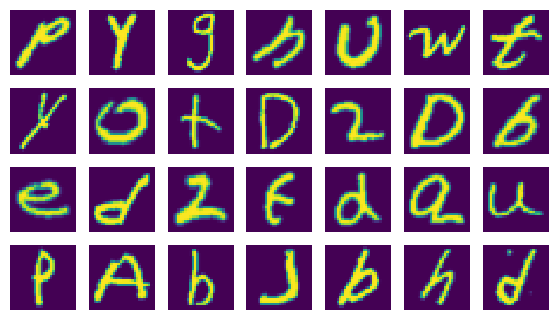
\includegraphics[scale=0.4]{emnist_letters}
	\caption[EMNIST-Letters datasets]{EMNIST-Letters dataset}\label{Abb:emnist_letters}
\end{figure}

The kaggle A-Z dataset has been released by the kaggle user Sachin Patel to an easy to read csv file. 
It contains only uppercase letters rescaled to be images with 28x28 pixels. 
It has a traning with 362.450 images and a test set with 10.000 images.
The goal of creating this dataset was to help beginners to do their first step in the deep learning. 
It is also the reason why it was used at the beginning of this project.  
But because it contains only uppercase letters, it was asumed that, in combination with other datasets, 
the prediction results of texts with lower and upper case letters will be incorrect due to the randomization of these letters. 
In this case, the target of this project could not be fulfilled and other datasets were chosen to move forward. 

\subsubsection{Alpha-numerical datasets}
For a handwritten text containing both letters and digits, a recognition can be performed using the following datasets: 

\begin{itemize}
    \item EMNIST-balanced dataset
    \item EMNIST-byMerge dataset.
  \end{itemize}

\noindent
The EMNIST-byMerge dataset has more data and an inconstant number of images per class compared to 
EMNIST-balanced dataset. 
The EMNIST-balanced is made up of 112.800 images in the training set and 18.800 images in the test set. 
Likewise the EMNIST-byMerge contains 697.932 images in the training set and 116.323 images in the test set. 
Both of them have 47 classes with some lowercase letters missing (for example: c/C, o/O, s/S). 
The deletion of this letters avoids the confusion due to the similarity of theirs lower and upper case shapes. 
This solves the classification issues while predicting. 
\hfill \break

\noindent
The visual breakdown of these two datasets is illustrated in the figure(\ref{Abb:visual_breakdown}).

\begin{figure}[htb]
	\centering
	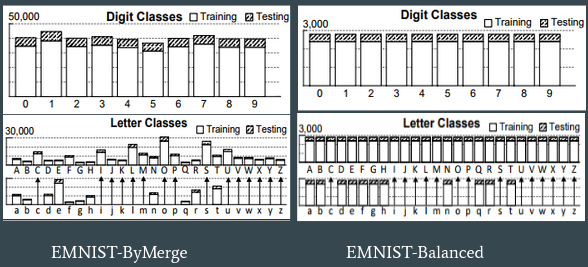
\includegraphics[width=0.7\textwidth]{visual_breakdown}
	\caption[Text datasets]{Visual breakdown of EMNIST-balanced and byMerge datasets(\cite{[2]})} \label{Abb:visual_breakdown}
\end{figure}

The deletion by both datasets is represented on this figure with a vertically directed arrow.

\noindent
Some example of images in these datasets are shown in the figure(\ref{Abb:balanced_and_byMerge}).

\begin{figure}[htb]
	\centering
	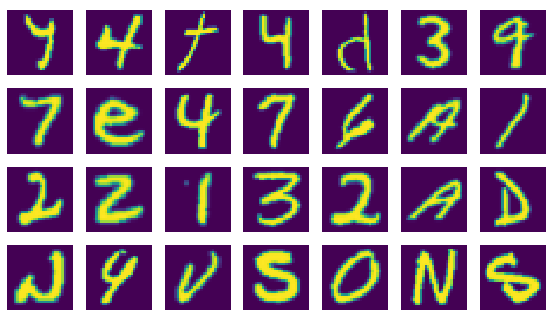
\includegraphics[scale=0.4]{demo_emnist_by_merge}
	\caption[Text datasets]{EMNIST-balanced and byMerge datasets}\label{Abb:balanced_and_byMerge}
\end{figure}

\newpage
\subsection{Own built dataset}
Despite the fact that, ready-for-use datasets provide a big choice of data, a custom dataset was created to fulfill the goal 
of this project. 
The name given to this dataset is \emph{SWTP-AI dataset}.
It contains diacritical letters, characters and some text ponctuations, written in form of a text paper with
fifteen(15) different handwritings. 
Detailed steps on how this dataset was built will be explained in the chapter "training\_guide\_tesseract". 
An example of the content of this dataset is in the picture (\ref{Abb:SWTP_KI_dataset}) below:

\begin{figure}[htb]
	\centering
	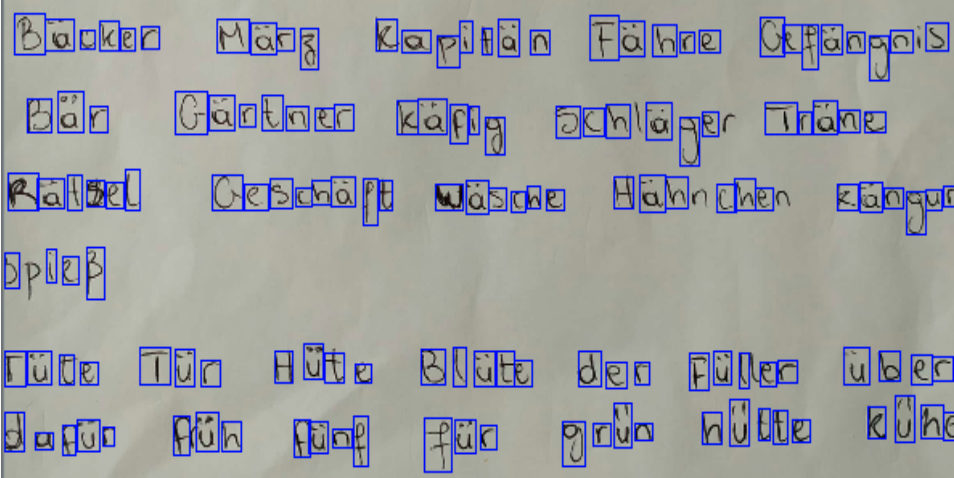
\includegraphics[width=0.7\textwidth]{swtp_ki_dataset}
	\caption[custom dataset]{SWTP-AI dataset}\label{Abb:SWTP_KI_dataset}
\end{figure}